\chapter{Тестирование алгоритмов}
Для тестирования разработанных алгоритмов сжатия данных были использованы исторические данные о температуре воздуха в Санкт-Петербурге.

\begin{figure}[ht]
    \centering
    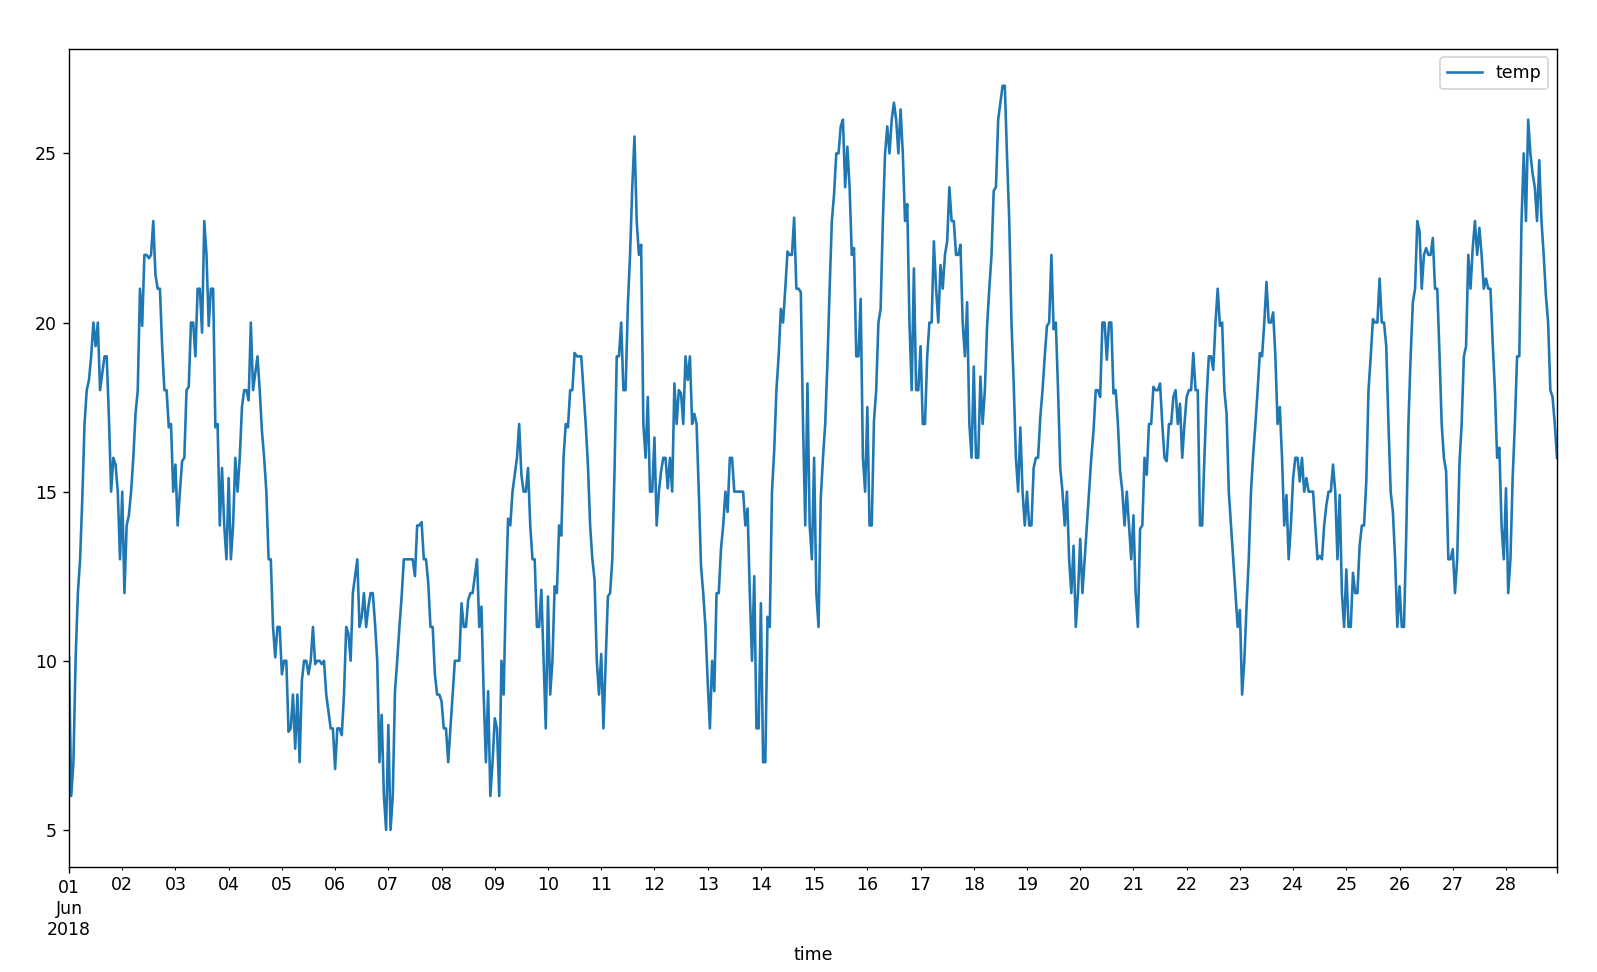
\includegraphics[width=1\textwidth]{spb_dataset.png}
    \caption{Почасовая температура в Санкт-Петербурге в июне 2018 года}
    \label{fig:spb_dataset}
\end{figure}

Алгоритмы были протестированы на предмет эффективности сжатия и потери данных.
Данные о температуре были получены с помощью библиотеки meteostat, которая предоставляет доступ к метеорологическим данным. В данном случае были использованы почасовые данные о температуре воздуха в Санкт-Петербурге за период с 1 июня 2018 года по 28 июня 2018 года. \\

Исходный код для тестирования алгоритмов:

\begin{lstlisting}[language=python, caption=Исходный код для тестирования алгоритмов, captionpos=b, frame=single]
from k_rle import k_rle_code, k_rle_decode
from ltc import ltc_code

from datetime import datetime
from meteostat import Hourly, Point
import numpy as np
import matplotlib.pyplot as plt
import time

def create_temperature_stream(multiplier: int, with_timestamps = False):
    start = datetime(2018, 6, 1)
    end = datetime(2018, 6, 28, 23, 59)
    saint_petersburg = Point(59.9387, 30.3256, 10) 
    data = Hourly(saint_petersburg, start, end)
    data = data.fetch()
    stream = []
    if not with_timestamps:
        for temp in data['temp']:
            stream.append(int(temp * 1e7))
    else:
        for i, item in enumerate(data['temp']):
            stream.append( (int(data.index.get_level_values("time")[i].timestamp()),
             item) )
    return stream
    
def test_k_rle():
    multiplier = 1e7
    source_stream = create_temperature_stream(multiplier)
    i_values = []
    compress_rates = []
    data_losses = []
    for i in range(1, 500 + 1, 10):
        coded_stream = k_rle_code(source_stream, multiplier * i / 100)
        decoded_stream = k_rle_decode(coded_stream, 2048)
        compress_rate = int((1 - (len(coded_stream) / len(source_stream))) * 100)
        data_loss = np.mean( np.array(source_stream) != np.array(decoded_stream) )*100
        
        i_values.append(i / 100)
        compress_rates.append(compress_rate)
        data_losses.append(data_loss)
        
        print('-------------------------------')
        print(f'i = {i / 100}, compress_rate = {compress_rate}%, loss = {data_loss}%')
        print('-------------------------------')
        
    plt.figure(figsize=(10, 5))

    plt.subplot(1, 2, 1)
    plt.plot(i_values, compress_rates)
    plt.title('Compression Rate vs i')
    plt.xlabel('i')
    plt.ylabel('Compression Rate (%)')

    plt.subplot(1, 2, 2)
    plt.plot(i_values, data_losses)
    plt.title('Data Loss vs i')
    plt.xlabel('i')
    plt.ylabel('Data Loss (%)')

    plt.tight_layout()
    plt.show()    
    
def test_ltc():
    multiplier = 1e7
    source_stream = create_temperature_stream(multiplier, with_timestamps=True)
    i_values = []
    compress_rates = []
    for i in range(1, 500 + 1, 10):
        coded_stream = ltc_code(source_stream, i / 100)
        compress_rate = int((1 - (len(coded_stream) / len(source_stream))) * 100)
        
        i_values.append(i / 100)
        compress_rates.append(compress_rate)
        
        print('-------------------------------')
        print(f'i = {i / 100}, compress_rate = {compress_rate}%')
        
    plt.figure(figsize=(5, 5))
    plt.subplot(1, 2, 1)
    plt.plot(i_values, compress_rates)
    plt.title('Compression Rate vs i')
    plt.xlabel('i')
    plt.ylabel('Compression Rate (%)')
    plt.tight_layout()
    plt.show()   

if __name__ == '__main__':
    test_k_rle()
    test_ltc()
\end{lstlisting}

\endinput
